\chapter{Biological background}
In this chapter we will present basic biological terms, which we will use later in this work.
We will describe molecules performing functions in living organisms and their representation in bioinformatics and computational biology.
We will explain relationships between these molecules, which will support our method later.

\section{Biological molecules}

\subsection{Deoxyribonucleic acid}
Deoxyribonucleic acid (DNA) is a long chain of nucleotides (bases) of four types - adenine, cytosine, guanine and thymine.
These bases are connected through a phosphodiester bond, connection between the 3' carbon atom of one deoxyribose and the 5' carbon atom of the second deoxyribose.
The structure of DNA consists of two complementary strands coiled around each other in the form of a double helix.
In this double helix adenine is paired with thymine and cytosine with guanine through hydrogen bonds.

In bioinformatics and computational biology, we usually represent a base by its first letter - A for adenine, C for cytosine, G for guanine and T for thymine.
Due to linear organisation of nucleotides, a DNA molecule can be represented as a word from alphabet \{A, C, G, T\}, called DNA sequence. We usually store biological sequences in simple plain text files.
Probably the most commonly used format is the FASTA format.
It can consist of one or multiple records, each representing a single DNA sequence.
Each record starts with the identifier of the sequence, which is followed by lines of the DNA sequence written in direction from 5' to 3'.

\subsection{Ribonucleic acid}
Ribonucleic acid (RNA) is, similar to DNA, it is a polymeric molecule consisting of four types of nucleotides.
There are three main differences between DNA and RNA molecules.
Firstly, the sugar-phosphate backbone of RNA contains ribose instead of deoxyribose.
This change in structure makes RNA less stable as it is more prone to hydrolysis.
Another distinctive feature of RNA is that it contains uracil instead of thymine.
Additionally, RNA appears in nature mostly as a single-stranded molecule, whereas DNA is mostly double-stranded.
This characteristic allows RNA to form more complex structures and show enzymatic activity.
In bioinformatics, sequences of RNA are usually written, similarly as with DNA, from 5' to 3', with the difference of U for uracil instead of T for thymine.

\subsection{Protein}
Proteins are polymers consisting of amino acids connected by a peptide bond.
There are 20 basic proteinogenic amino acids encoded in DNA sequences and 2 proteinogenic amino acids incorporated into proteins by a unique mechanism.
Protein performs overwhelming majority of functions in living organisms.
Thanks to this characteristic, they will be of high importance in our analysis.
In bioinformatics, protein sequences are represented as a string of 1-letter abbreviations of their amino acids. All proteinogenic amino acids with their 1-letter codes can be found in the Table (\ref{tab:amino})

\begin{table}
 \centering
        \begin{tabular}{ l  l  l  l }
         \hline
         amino acid & 1-letter code & amino acid & 1-letter code \\
         \hline  
         alanine & A & arginine & R \\
         asparagine & N & aspartic acid & D \\
         cysteine & C & glutamine & Q \\
         glutamic acid & E & glycine & G \\
         histidine & H & isoleucine & I \\
         leucine & L & lysine & K \\
         methionine & M & phenylalanine & F \\
         proline & P & serine & S \\
         threonine & T & tryptophan & W \\
         tyrosine & Y & valine & V \\
         selenocysteine & U & pyrrolysine & O \\
         \hline
        \end{tabular}
        \caption{Amino acids}
        \label{tab:amino}
\end{table}



\section{Central dogma of molecular biology}
Central dogma of molecular biology explains relationships between biological molecules described in previous sections.
Most organisms store their genetic information in the form of DNA.
Some parts of DNA, usually called genes, are transcribed into RNA.
Afterwards, ribosome translates the RNA sequence into a protein that is based on the RNA codon table.
Proteins are then folded into their natural 3D structure and prepared to realize their corresponding functions.

We based our work on the central dogma of molecular biology and on the assumption that genes will be useful indicators when predicting the biological trait, the ability to infect certain hosts.

\begin{figure}[htp]
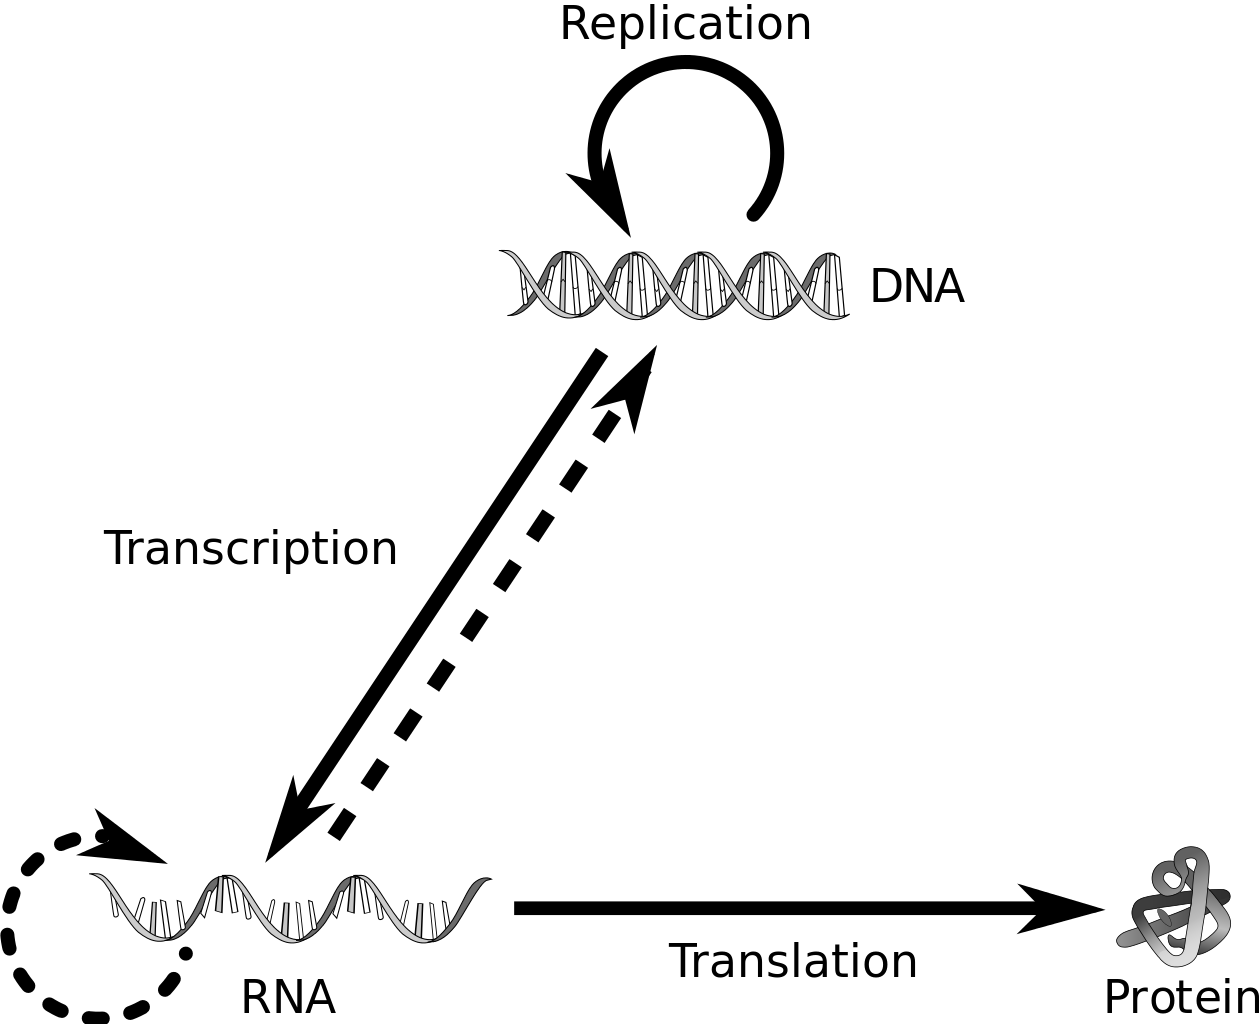
\includegraphics[width=\linewidth]{./images/central_dogma.png}
\centering
\caption{Central dogma of molecular biology[h]}
\end{figure}
